\documentclass[11pt]{article}
\usepackage{geometry}
\geometry{a4paper}
\usepackage{graphicx,amsmath,amssymb,bm,enumerate,booktabs,minted,indentfirst,enumitem}
\usepackage{pdflscape,multirow}

\usepackage[colorlinks]{hyperref}
% 中文排版\
\usepackage[BoldFont,SlantFont,fallback]{xeCJK}
\setCJKmainfont{simsun.ttf}
\setCJKsansfont{simhei.ttf}
\setCJKmonofont{simfang.ttf}

\linespread{1.3}
\setlength{\parindent}{2em}
\setenumerate{itemsep=0pt}

\title{Explorations on Building a Cache System \\ Based on Racetrack Memory}
% \subtitle{RaceTrack Cache simulator design and system optimization}
\author{杨俊睿 1200012860 \\
刘当一 1100011625}
\date{}

\begin{document}
\maketitle


\section{Introduction}

The wide adoption of chip multiprocessors (CMPs) has generated an explosive demand for on-chip memory resources. Unfortunately, as technology scaling continues, the reliance on conventional SRAM technology for on-chip caches raises several concerns including the large memory cell size, the high leakage power consumption, and the low resilience to soft errors. A very recent emerging nonvolatile memory technology, the racetrack memory, has been projected to over come the density barrier and high leakage power of existing memory solutions.

In this homework we proposed serveral optimization that can imporve the performance of current racetrack memory act as computer's cache. We design a simulator for racetrack cache and implement some idea on it.


\section{Basics of Racetrack Memory}

Figure \ref{fig:struct} showed a basic structure of a racetrack strip, which consist of a nano wire and several reading and writing port. The nano wire has many magnetic domains, where the information stores at, and they are separated by narrow domain walls for prevention of wrong access. The nano wire is driven by shift ctrl, allowing the information stored inside those domains to shift across the nano wire. Some access port is placed across the nano wire in order to read and write data on the wire. Typically, because of the large size of access ports comparing to the domains on the nano wire, there are much more domains than access ports. Traditionally, only RW-port is build enabling both write and read access to the domains. Recent development propose R port and W port in a smaller size for more flexibility in design.

\begin{figure}
\centering
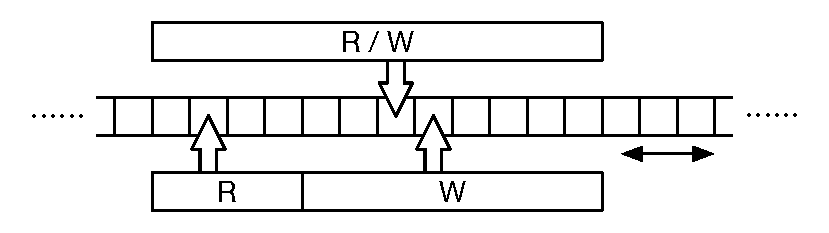
\includegraphics{fig1.pdf}
\caption{Basic structure of a racetrack strip}
\label{fig:struct}
\end{figure}


\section{Design}

\subsection{Design of simulator}

\begin{figure}
\centering
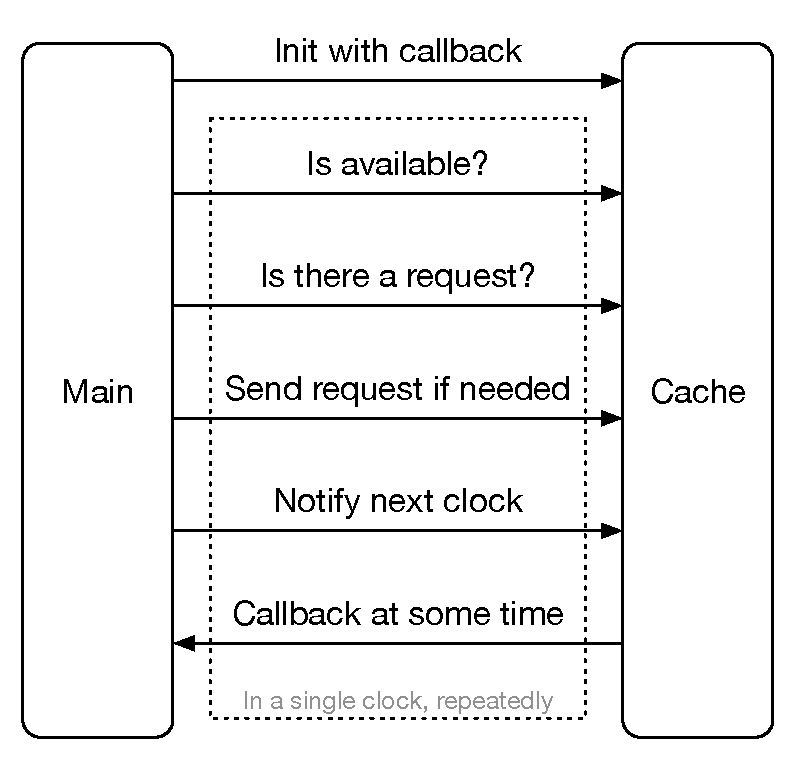
\includegraphics[width=260pt]{fig2.pdf}
\caption{Design of simulator}
\label{fig:design1}
\end{figure}

Our simulator exactly mimic the CPU cache interaction. Our simulator is composed of two parts as depicted in Figure 2. The part on the left is the main simulation sequence control logic in \texttt{main} function, which send the request recorded in trace file in the exact same order and time. The part on the right is the cache module, which have different implementation for different cache. All cache module inherit a base class called as \texttt{BaseCache}.

\subsection{Design of cache}

\begin{figure}
\centering
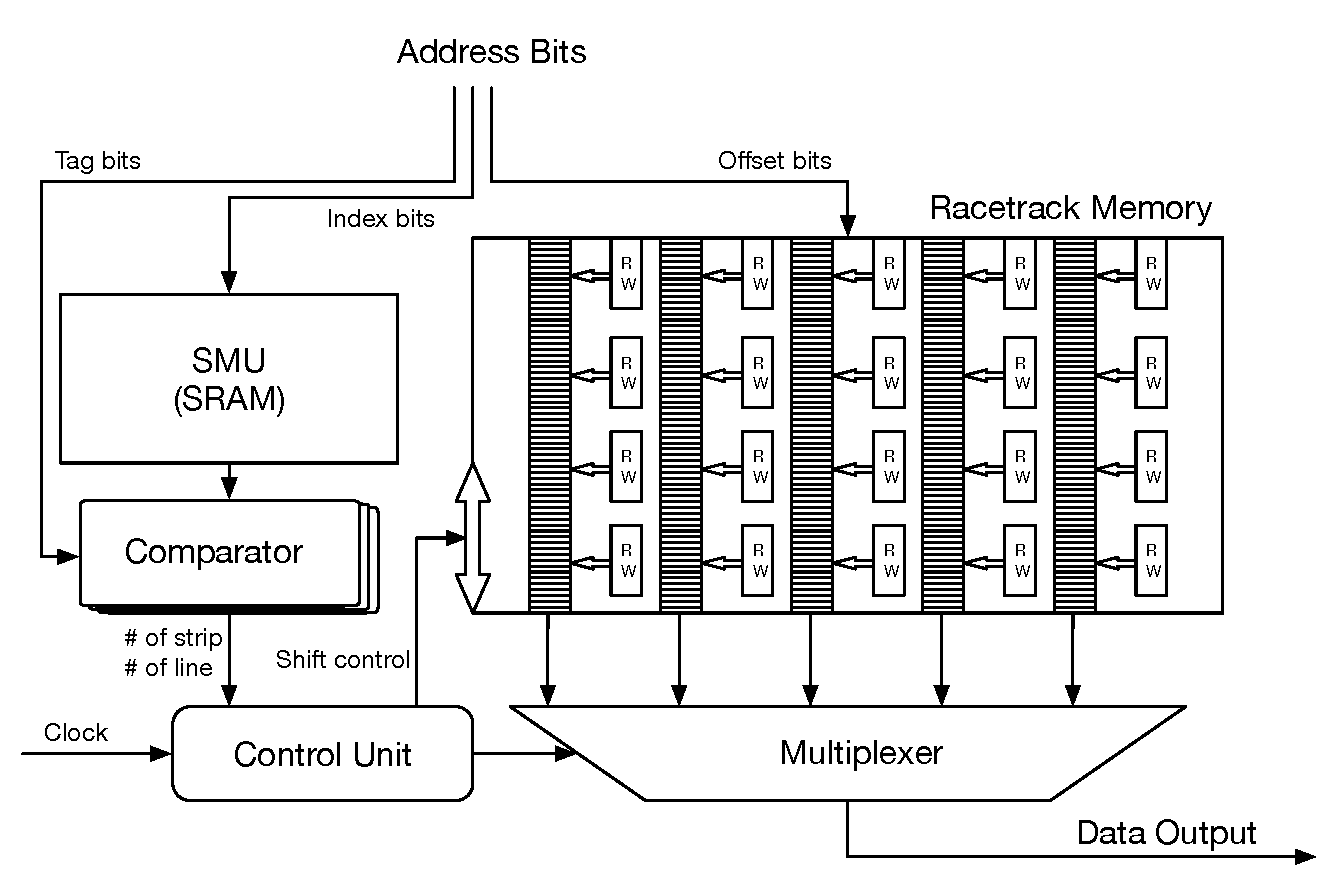
\includegraphics[width=400pt]{fig4.pdf}
\caption{Design of cache}
\label{fig:design2}
\end{figure}

We adopted a common design of hybrid cache (consist of both SRAM and racetrack memory) (figure 3). A cache is composed of 3 parts: SMU (strip mapping unit), Racetrack memory (for actual storage) and Control unit. 

\begin{itemize}

\item SMU is mainly consist of a small piece of SRAM comparing to the much larger capacity of racetrack memory. SMU is in charge of recording the tag bits of each cache line and provide a random access interface of determine the availability and the location on racetrack strips of a specific memory address.

\item Racetrack memory is the main storage device for cache, it storage all the data of the address cached.

\item Control unit is in charge of memory access, racetrack shift and read or write action performed on strips. Our control unit is designed to work like a multi cycle computing device. The control unit has a faster internal clock to organize internal work, jobs likes shift, read or write might cost more internal clock while tasks like SMU look up might just cost a fraction of a cycle.
\end{itemize}

There is some improvement can be done on this architecture.

\subsubsection{Static Strategy}

\begin{itemize}
\item ``Hybird Port''

We never need to read and write or write and read a same cell in a row, we believe placing a RW port whose length equals a read and write port combination would be a waste. For example, in IdleSort strategy, we might want to swap neighbour cell content to align the content in a bubblesort way. In this case, a read and write port combination with aside port can reach 2 cycle / swap and a RW port can only achieve 3 cycle / swap.

\item ``Massive Read Port'' and ``Swap port''

Because read operation is often on critical path for computing. We can significantly increase the profromance by increase the read port while maintain the same number of write port.

``Swap port'' is a combination of a pair of adjoining read and write port with their port also placed together. As steated in ``Hybird Port'' section, this enable fast bubble-sort used in ``Idle Defragment'' section.

\item Set placement across group

We prefer placing neighboor set in different group, as they are often accessed together. This allow the first access to shift first group while the group for the group for second access is still remain in their best position and unaffected by the first access.

\end{itemize}

\subsubsection{Dynamic Strategy}

\begin{itemize}
\item Tape header management

We choose a ``Eager'' policy: the port always return to an optimal positon after each access. This decision is basis for many other strategy we adopted below.

\item ``Set Reampping''

We deploy additional bit in tag array to store the address accross the same group. Thus, a cache line in a set can be remapped to anywhere in the group while maintain same time for tag comparasion.

\item ``Lazy Evict''

When a cache miss is generated, we will immediately return the data from the main memory to CPU without evict the corrispond cell. The COU will preform the evict action then.

\item ``Idle Defragment''

We discovered that cell around the position of read port can be accessed faster. Thus, we want the more likely-to-be-accessed cache line be placed near the read port. Fortunately, the history data stored for evict decision can also be used to decide optimal position for each cache line in cell.

``Idle Defragment'' is a action performed during idle period to maintain the most optimal placement (most used cell ) for each cell. Also, It must be able to be interrupted smoothly when CPU access a data in the group being defragmenting.

\item (``Shift Predictor'')

We can maintain a ``Shift Prediction Table'' for each cell in group, recording next access position to the same group. This strategy is conflict with most strategies mentioned above and might not be adopted.

\item ``Dual Channel''

We observe that each access may come with one swap to maintain the order. Swap between two group cost significantly less than swap in one group. Thus, we futher add one bit to address bits in tag array to enable each set to be placed across two group.

\end{itemize}

\subsection{Implementation of cache}

\subsubsection{Common Specification}

Size characteristic

\begin{center}
\begin{tabular}{llll}
\toprule
Cache size & Strips group count & Strips count in each group & Bits on each strip \\
\midrule
4M         & 1024               & 512                        & 64 \\
\bottomrule
\end{tabular}
\end{center}

Timing characteristic

\begin{center}
\begin{tabular}{llll}
\toprule
Miss penalty & Read duration & Write duration & Shift duration \\
\midrule
100          & 1             & 1              & 1             \\
\bottomrule
\end{tabular}
\end{center}

Physical characteristic

\begin{center}
\begin{tabular}{lll}
\toprule
Read Port & Write Port & RW Port \\
\midrule
4         & 8          & 12     \\
\bottomrule
\end{tabular}
\end{center}

\subsubsection{Baseline cache}
Baseline cache is a cache design given on the class. The cache have the following characteristics: 
\begin{itemize}
\item replacement policy: LRU
\item cache associativity: 8
\item port arrangement: 4 RW port equally distributed on the strip
\end{itemize}

The baseline use a very intrinsic way to index each group on port. The 0--7 group is located on the 1st strip and so on.

This cache adopt a simple head management policy generally called as lazy policy. The position of each strip is left as is after each read or write process.

\subsubsection{Eager cache}

Eager cache maintain most characteristics of baseline cache, but adopt a more evolved head management policy, eager policy. When eager policy is used, cache head is always tends to return to its original position when the cache is free.

\subsubsection{Massive cache}

Massive cache change the port arrangement (Figure \ref{fig:massive}). In this arrangement massive amount of read port is used. 16 read port is equally distributed on the strip the first and the last one also perform as a write port.

\subsubsection{Comments}

Although we proposed many optimizations above, but we found that the massive cache perfectly solve the problem of too many shift caused by cache access. The origin of the latency is mostly came from miss penlty and stall (CPU cannot send any request to cache because cache is busy handling other requests whose result might have already been returned).

\begin{figure}
\centering
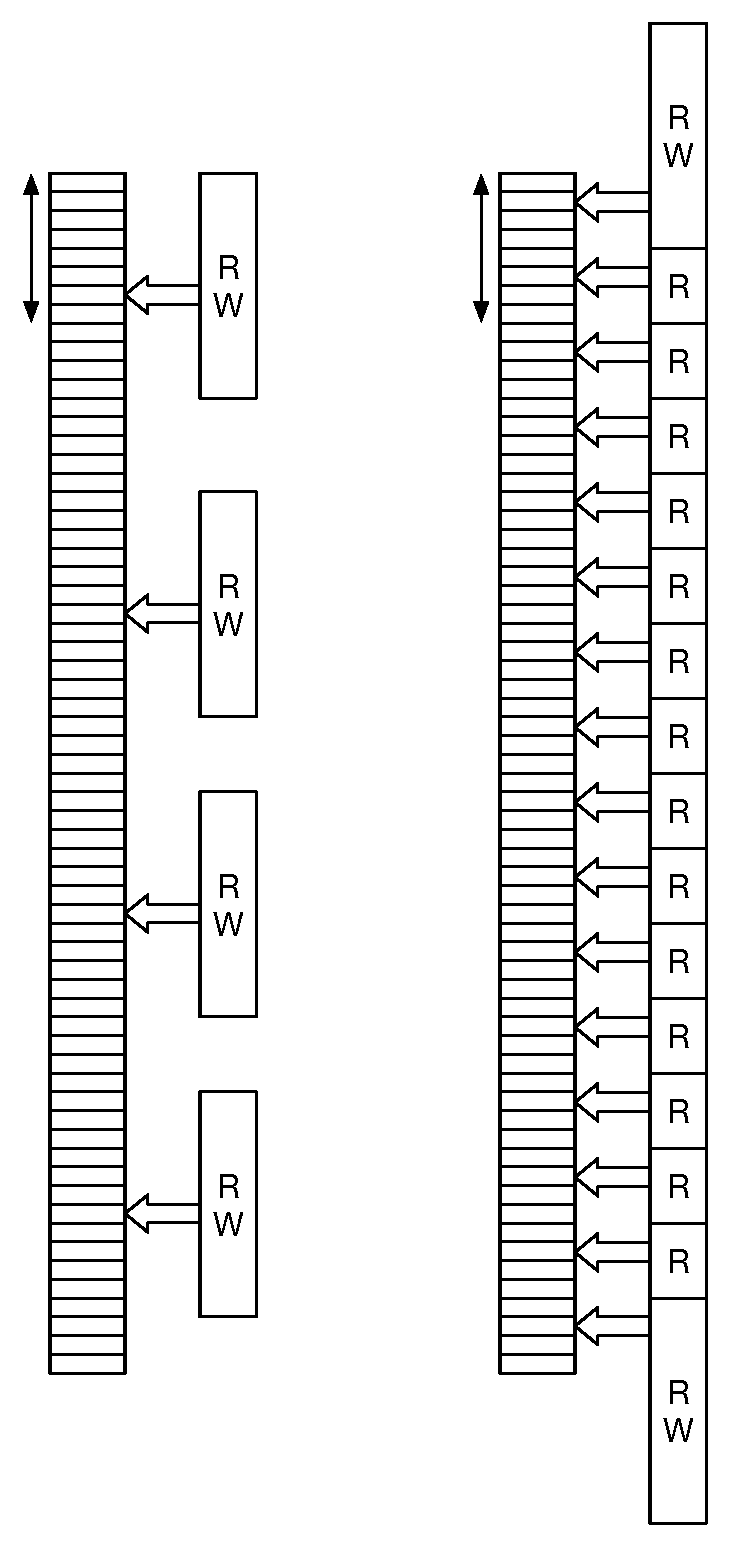
\includegraphics[height=400pt]{fig3.pdf}
\caption{Difference between baseline cache and massive cache}
\label{fig:massive}
\end{figure}

\section{Implementation}

\subsection{\texttt{main} function}

The \texttt{main} function receives multiple kind of arguments. It can run the simulator or just do an analysis of the trace file, which includes the percentage of R/W, the average interval between two request and the average hit times per address. After running the simulator, it prints the statistics data including average delay, average shift times and miss rate. Following is the pseudocode of main.

\begin{minted}[frame=lines, linenos]{c++}
int main() {
    vector<Request> requests = read_from_trace();
    if (analysis) {
        do_analysis(requests);
        exit(0);
    }
    BaseCache cache = initial_cache_with_callback([&](Request req){
        total_delay += current_tick - req.start_tick;
        success_request_count++;
    });
    auto it = requests.begin();
    while (success_request_count < requests.size()) {
        if (cache.isAvailable() && it != requests.end() &&
            it->start_tick + 6 <= current_tick) {
            cache.requestCache(*it);
            it++;
        }
        current_tick++;
        cache.nextTick(current_tick);
    }
    print_statistics();
}
\end{minted}

\subsection{Interface defined in \texttt{BaseCache}}

Below is code adopted from \texttt{BaseCache.hh}.

\begin{minted}[frame=lines, linenos]{c++}
class BaseCache {
public:
    typedef std::function<void(Request)> callback_type;
    BaseCache(callback_type callback) : callback(callback) {}
    virtual void nextTick(Tick) = 0;
    virtual void requestCache(Request) = 0;
    virtual bool isAvailable() = 0;
#ifdef STAT
    virtual std::string getStateName() = 0;
#endif
protected:
    callback_type callback;
    static const Tick missPenalty = 100;
    static const Tick accessLatency = 6;
};
\end{minted}

\subsection{Cache Implementation}

As stated above, we use a finite state machine to specify what should be done in each cycle. Each state of the FSM cost different time.

The state is stored in enum class \texttt{State}

\begin{minted}[frame=lines, linenos]{c++}
typedef enum : uint8_t {
    StateIdle,
    StateMoving,
    StateReading,
    StateLookup,
    StateMiss,
    StateWriting,
} State;
\end{minted}

Function \texttt{nextTick} is used to determine all the state change in one cycle:

\begin{minted}[frame=lines, linenos]{c++}
void BaselineCache::nextTick(Tick tick)
{
    for (int64_t currentMicroTickLeft = microTickPerTick;
        currentMicroTickLeft >= stateLength(state);) {
        currentMicroTickLeft -= stateLength(state);
        nextState(tick);
    }
}
\end{minted}

Function \texttt{nextState} is called if there is enough time for next State this cycle.

\begin{minted}[frame=lines, linenos]{c++}
void BaselineCache::nextState(Tick tick)
{
    switch (state) {
    case StateIdle:
        break;
    case StateMoving: {
        ...
    }
    case StateReading: {
        ...
    }
    case StateWriting: {
        ...
    }
    case StateLookup: {
        ...
    }
    case StateMiss: {
        ...
    }
    }
}
\end{minted}

One example of FSM used in cache simulator is shown in Figure \ref{fig:auto}.


\begin{figure}[h]
\centering
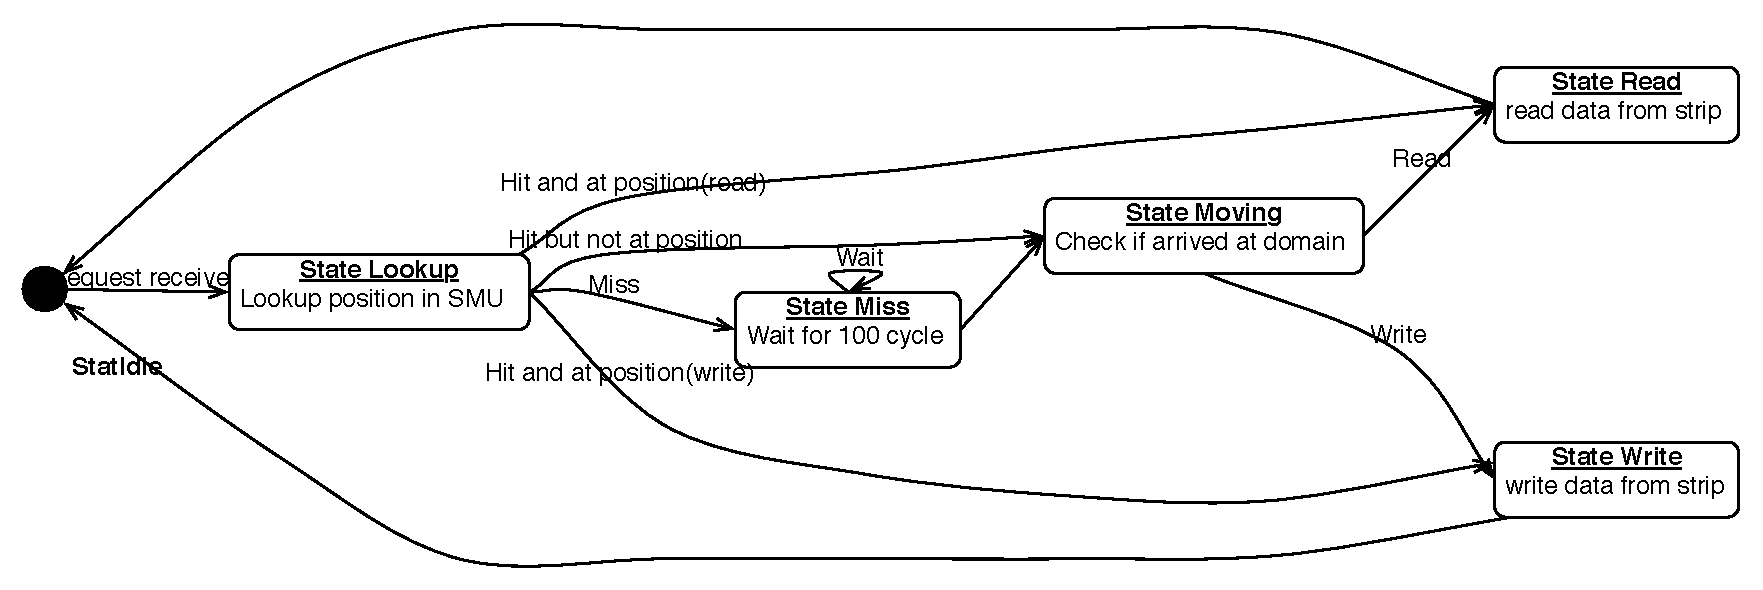
\includegraphics[width=400pt]{fig5.pdf}
\caption{FSM}
\label{fig:auto}
\end{figure}


\section{Experiment}

We have conducted a series of experiment about all three cache listed above. We used L2 cache trace of serveral benchmarks adopted from spec2006. Table \ref{tab:big} shows the results.

\newgeometry{margin=20pt}
\begin{landscape}
\thispagestyle{empty}
\begin{table}
\begin{tabular}{lllllllllll}
\toprule
\multicolumn{1}{c}{\multirow{2}{*}{\begin{tabular}[c]{@{}c@{}}Trace\\ name\end{tabular}}} & \multicolumn{1}{c}{\multirow{2}{*}{\begin{tabular}[c]{@{}c@{}}Total\\ request\end{tabular}}} & \multicolumn{1}{c}{\multirow{2}{*}{\begin{tabular}[c]{@{}c@{}}Read \\ percentage\end{tabular}}} & \multicolumn{1}{c}{\multirow{2}{*}{\begin{tabular}[c]{@{}c@{}}Write \\ percentage\end{tabular}}} & \multicolumn{1}{c}{\multirow{2}{*}{\begin{tabular}[c]{@{}c@{}}Average \\ interval\end{tabular}}} & \multicolumn{2}{c}{BaselineCache}                                     & \multicolumn{2}{c}{EagerCache}                                        & \multicolumn{2}{c}{MassiveCache}                                      \\
\multicolumn{1}{c}{}                                                                      & \multicolumn{1}{c}{}                                                                         & \multicolumn{1}{c}{}                                                                            & \multicolumn{1}{c}{}                                                                             & \multicolumn{1}{c}{}                                                                             & \multicolumn{1}{c}{Average delay} & \multicolumn{1}{c}{Average shift} & \multicolumn{1}{c}{Average delay} & \multicolumn{1}{c}{Average shift} & \multicolumn{1}{c}{Average delay} & \multicolumn{1}{c}{Average shift} \\
\midrule
400.perlbench                                                                             & 264414                                                                                       & 81.16\%                                                                                         & 18.84\%                                                                                          & 72.6016                                                                                          & 14.3777                           & 5.56267                           & 12.05                             & 3.25196                           & 9.65834                           & 0.649663                          \\
401.bzip2                                                                                 & 3239378                                                                                      & 38.01\%                                                                                         & 61.99\%                                                                                          & 103.713                                                                                          & 12.7338                           & 2.85217                           & 11.4041                           & 1.52258                           & 10.9316                           & 0.137676                          \\
403.gcc                                                                                   & 2302351                                                                                      & 75.10\%                                                                                         & 24.90\%                                                                                          & 88.9929                                                                                          & 12.7161                           & 4.46245                           & 11.2373                           & 2.97328                           & 9.15914                           & 0.657313                          \\
410.bwaves                                                                                & 10564779                                                                                     & 10.64\%                                                                                         & 89.36\%                                                                                          & 34.4297                                                                                          & 70.4803                           & 0.118944                          & 79.863                            & 0.252474                          & 100.352                           & 0.119173                          \\
429.mcf                                                                                   & 204593                                                                                       & 24.39\%                                                                                         & 75.62\%                                                                                          & 504.864                                                                                          & 10.3015                           & 0.809368                          & 10.091                            & 0.644611                          & 9.92874                           & 0.175827                          \\
434.zeusmp                                                                                & 1604122                                                                                      & 1.12\%                                                                                          & 98.88\%                                                                                          & 143.167                                                                                          & 7.83995                           & 0.0639689                         & 7.57755                           & 0.0386367                         & 8.08585                           & 0.0156622                         \\
435.gromacs                                                                               & 1903172                                                                                      & 98.90\%                                                                                         & 1.10\%                                                                                           & 65.2366                                                                                          & 15.0395                           & 7.90137                           & 11.0865                           & 3.95072                           & 8.12726                           & 0.987641                          \\
436.cactusADM                                                                             & 14290355                                                                                     & 0.49\%                                                                                          & 99.51\%                                                                                          & 105.339                                                                                          & 13.3592                           & 0.0211438                         & 13.3677                           & 0.0191517                         & 13.4803                           & 0.00424349                        \\
444.namd                                                                                  & 78250                                                                                        & 83.09\%                                                                                         & 16.91\%                                                                                          & 1176                                                                                             & 12.4915                           & 4.72725                           & 11.526                            & 3.77541                           & 8.58307                           & 0.792895                          \\
445.gobmk                                                                                 & 6035                                                                                         & 8.68\%                                                                                          & 91.32\%                                                                                          & 109.4                                                                                            & 15.968                            & 0.0493786                         & 15.0482                           & 0.0273405                         & 15.8949                           & 0.0064623                         \\
450.soplex                                                                                & 1762867                                                                                      & 55.77\%                                                                                         & 44.23\%                                                                                          & 96.082                                                                                           & 10.5724                           & 2.97053                           & 9.45271                           & 2.18203                           & 7.92938                           & 0.43692                           \\
453.povray                                                                                & 1313708                                                                                      & 69.88\%                                                                                         & 30.12\%                                                                                          & 111.882                                                                                          & 12.6788                           & 3.96841                           & 11.4343                           & 2.7483                            & 9.20951                           & 0.413756                          \\
456.hmmer                                                                                 & 12554235                                                                                     & 33.41\%                                                                                         & 66.59\%                                                                                          & 50.8927                                                                                          & 7.40245                           & 0.29512                           & 8.80732                           & 1.29228                           & 9.55611                           & 0.205747                          \\
458.sjeng                                                                                 & 9961508                                                                                      & 0.01\%                                                                                          & 99.99\%                                                                                          & 94.419                                                                                           & 8.17607                           & 0.000128495                       & 7.0045                            & 4.01E-05                          & 8.16028                           & 9.34E-06                          \\
459.GemsFDTD                                                                              & 471319                                                                                       & 99.86\%                                                                                         & 0.14\%                                                                                           & 220.096                                                                                          & 14.4753                           & 7.12547                           & 10.8803                           & 3.59422                           & 8.26813                           & 0.98714                           \\
462.libquantum                                                                            & 1388530                                                                                      & 0.01\%                                                                                          & 99.99\%                                                                                          & 140.374                                                                                          & 7.01023                           & 0                                 & 7.01023                           & 0                                 & 7.01025                           & 0                                 \\
464.h264ref                                                                               & 718961                                                                                       & 68.69\%                                                                                         & 31.31\%                                                                                          & 157.807                                                                                          & 11.6888                           & 4.2686                            & 10.2948                           & 2.84535                           & 8.42002                           & 0.742668                          \\
470.lbm                                                                                   & 8196221                                                                                      & 0.00\%                                                                                          & 100.00\%                                                                                         & 99.5596                                                                                          & 7.21586                           & 0                                 & 7.00012                           & 0                                 & 7.26163                           & 0                                 \\
471.omnetpp                                                                               & 2483572                                                                                      & 83.50\%                                                                                         & 16.50\%                                                                                          & 74.6604                                                                                          & 11.5974                           & 4.43903                           & 10.608                            & 3.39207                           & 7.96252                           & 0.61725                           \\
473.astar                                                                                 & 190291                                                                                       & 34.06\%                                                                                         & 65.94\%                                                                                          & 517.765                                                                                          & 9.07785                           & 1.1772                            & 9.38141                           & 1.53526                           & 8.45928                           & 0.200467                          \\
481.wrf                                                                                   & 2040346                                                                                      & 0.76\%                                                                                          & 99.24\%                                                                                          & 125.872                                                                                          & 7.207                             & 0.0403564                         & 7.18716                           & 0.0249845                         & 7.17751                           & 0.00596124                        \\
482.sphinx3                                                                               & 1875                                                                                         & 85.17\%                                                                                         & 14.83\%                                                                                          & 328.431                                                                                          & 63.9419                           & 1.77067                           & 63.7808                           & 1.6336                            & 62.488                            & 0.296533                         \\
\bottomrule
\end{tabular}
\caption{Experiment results}
\label{tab:big}
\end{table}
\end{landscape}
\restoregeometry

\section{Conclusion}
\subsection{Overall performance}
As shown in figure \ref{fig:con1}, in general, each generation of cache design have a better performance.

\begin{figure}
\centering
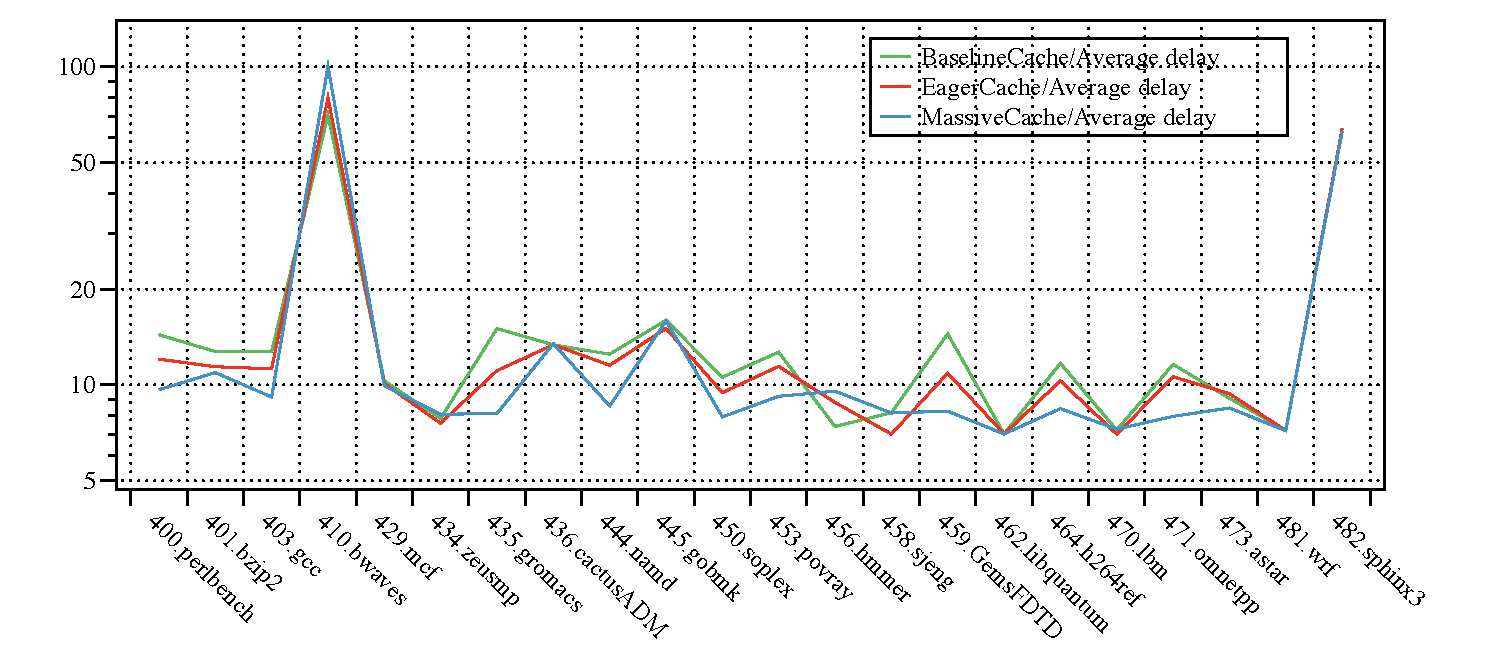
\includegraphics[width=400pt]{con1.pdf}
\caption{Comparsion of average delay}
\label{fig:con1}
\end{figure}

It is easier to observe the performance improvement if we only listed the average shift cycle of read access(figure \ref{fig:con2}) (write access is usually not on the critical path and therefore cause no direct performance impact\footnote{Although some benchmark who have very frequent access with many write accesses among them might witness a great reletivity between performance and write latency}).

\begin{figure}
\centering
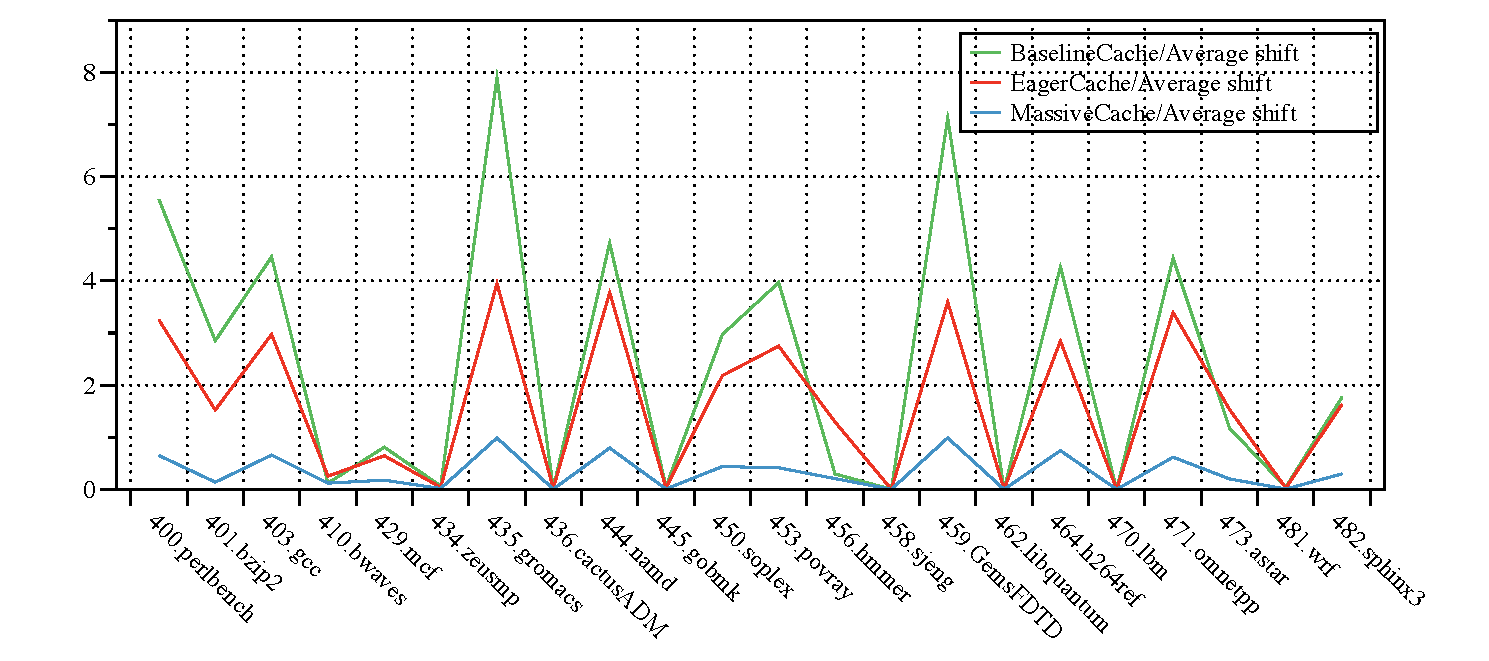
\includegraphics[width=400pt]{con2.pdf}
\caption{Comparsion of average shift}
\label{fig:con2}
\end{figure}

\subsection{In depth analysis}
We analysis some of the interesting experiment results and showed them here.

\subsubsection{410.bwaves.trace}

This trace have frequent cache access, while update and write access composed a large fraction of them. Total request number of this trace is 10564779 and 89\% of them are write access. The average interval of this trace is only 34 cycles, which means there is hardly engough time for the racetrack to return to its original position. This is a very well counter example of our plan, as we tends to overlook the latency of write access.

But in general, our practice have a promising result, as most of the trace is not as intensive as ``410.bwaves.trace'' and have smaller portion of write access among them.

\subsubsection{436.cactusADM.trace}
This trace also have frequent cache write access, but with larger interval, namely over 99\% of the access are write access but the average interval is over 100 cycle. This arrangement allow strips in racetrack cache to return to its original position after a write access when an effective eager policy is adopted. As a result only a slight performance is affected because of extra read ports replace some write ports.

\subsubsection{100.perlbench.trace}
This is an ideal example where our straegy of optimization works effectly. As seen in the table, perlbench have a low portion of write access and a abundent interval between each access. The massive amount of read port enable read access can be fulfilled even within one cycle, and write access will cause less problem as there is enough cycle for the strips to return to its position. The average delay reduced from 14 to 12 because of the adoption of eager policy and from 12 to 9.6 because of the adoption of massive read port policy.


\section{Future work}
Many work can still be done in this area, including:
\begin{itemize}
\item Implement remapping strategy to increase the number of write ports while maintain similar performance.
\item Try more ports distribution schemes and find the best one.
\item Try change the mapping location of memery address.
\end{itemize}
The same streagy we proposed on this cache system might also help improve the performance when racetrack memory is used as main memory. In fact, as the access to main memory is more regular and main memory has a lower rate of access, some of our strategy proposed in this homework migth have larger effect on the senerio where racetrack is used as main memory.

\newpage

\section*{References}

\begin{enumerate}
\item M. Mao, W. Wen, Y. Zhang, Y. Chen, and H. H. Li, ``Exploration of GPGPU Register File Architecture Using Domain-wall-shift-write based Racetrack Memory,'' presented at the DAC '14: Proceedings of the 51st Annual Design Automation Conference, New York, New York, USA, 2014, pp. 1–6.
\item Z. Sun, X. Bi, A. K. Jones, and H. Li, ``Design exploration of racetrack lower-level caches.,'' ISLPED, pp. 263–266, 2014.
\item R. Venkatesan, V. J. Kozhikkottu, C. Augustine, A. Raychowdhury, K. Roy, and A. Raghunathan, ``TapeCache: a high density, energy efficient cache based on domain wall memory.,'' ISLPED, pp. 185–190, 2012.
\end{enumerate}

\end{document}
